\chapter{Phương pháp VRAE: Vertical Residual Autoencoder}

Trong chương này, em trình bày chi tiết phương pháp VRAE (Vertical Residual Autoencoder), một kiến trúc nhẹ chuyên dụng cho bài toán khử nhiễu và khử mờ biển số xe. Mục tiêu của VRAE là duy trì fidelity (PSNR/SSIM), bảo toàn chi tiết vi mô, đồng thời đạt hiệu năng tính toán phù hợp cho ứng dụng thời gian thực trên ảnh có phần vùng quan tâm nhỏ.

\section{Tổng quan kiến trúc}
VRAE là một biến thể của Autoencoder với cấu trúc encoder–decoder chuẩn nhưng mở rộng bằng các khối residual theo chiều dọc và khối bổ trợ. Encoder sử dụng backbone dựa trên ResNet-50 (giữ cân bằng giữa năng lực biểu diễn và chi phí tính toán), trong khi decoder phục hồi ảnh sạch thông qua các lớp tích chập ngược (deconvolution).
\begin{figure}[H]
    \centering
    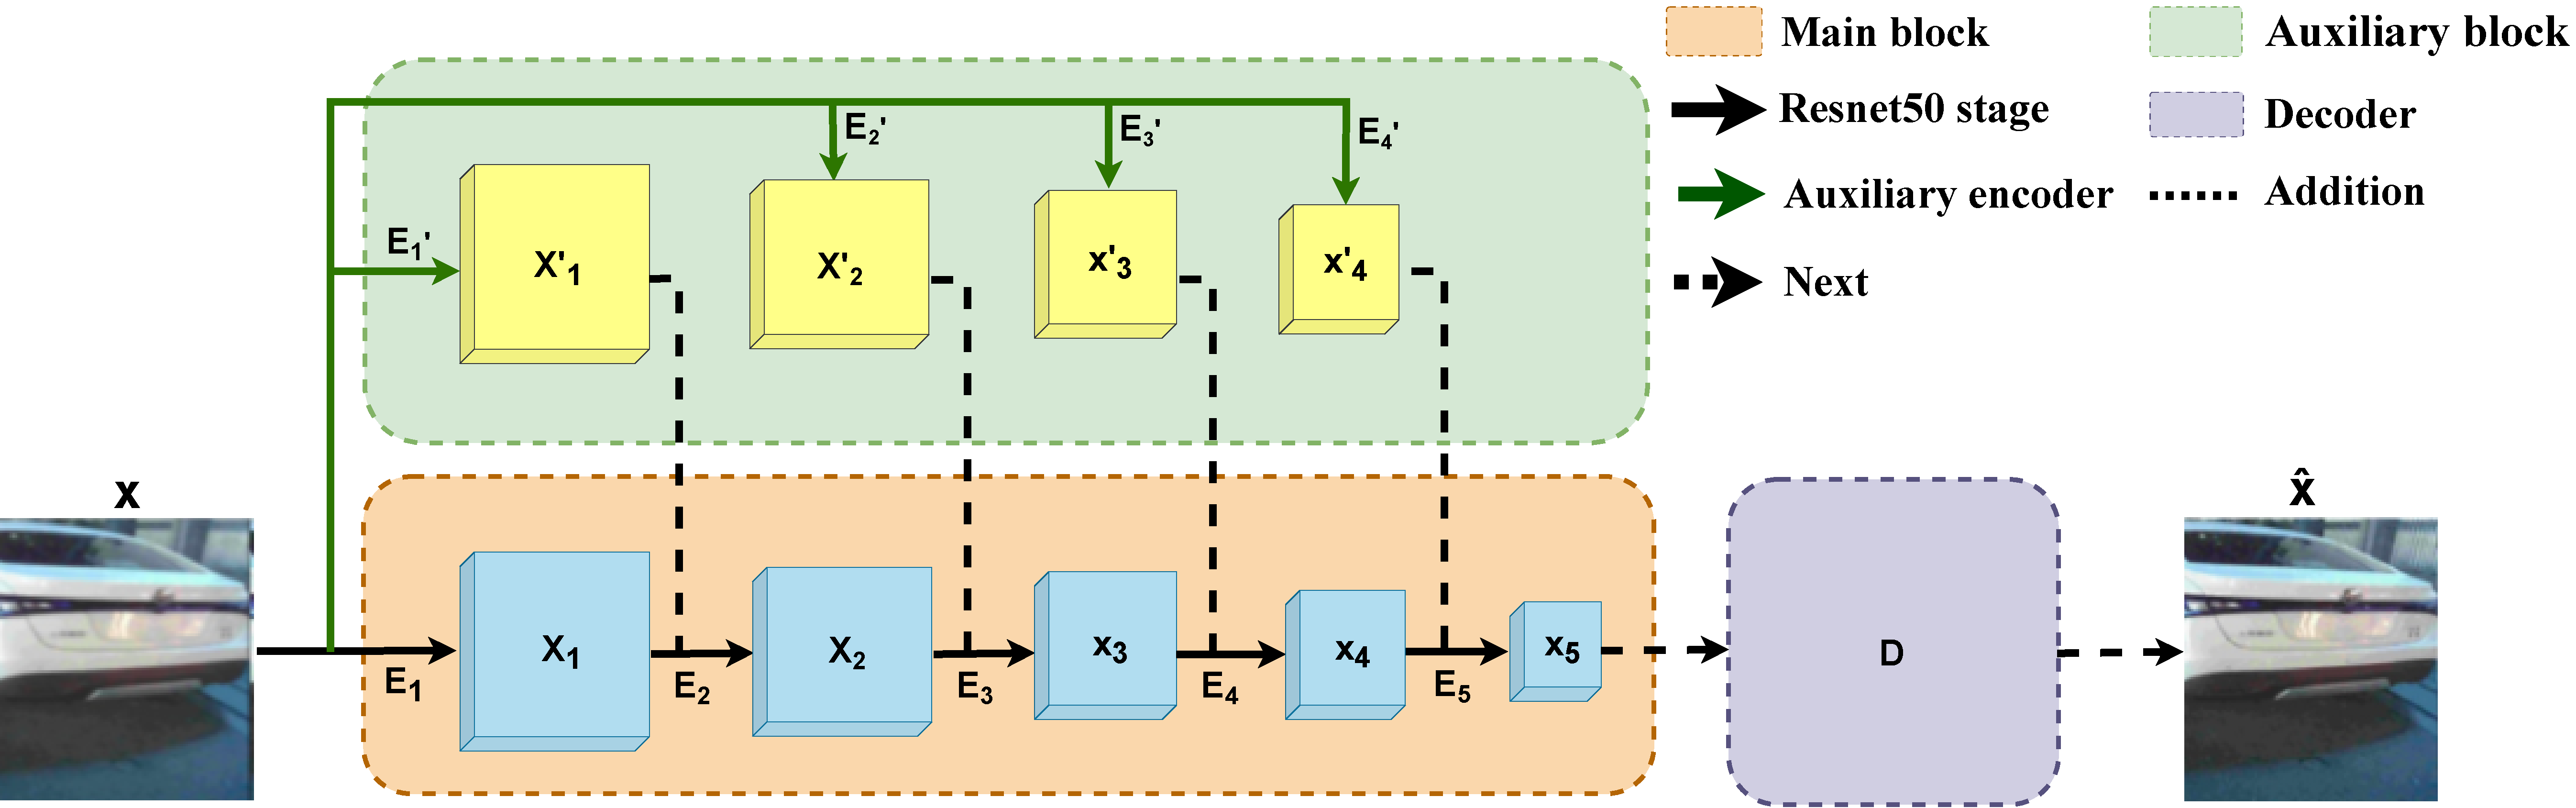
\includegraphics[width=1\linewidth]{images/VRAE.pdf}
    \caption{Kiến trúc phương pháp VRAE}
    \label{fig:VRAE_architecture}
\end{figure}

\subsection{Khối chính (Main Block)}
Khối chính là thành phần cốt lõi giúp bảo toàn và biến đổi thông tin theo trục dọc của kiến trúc. Trong thiết kế này, mỗi khối mã hóa chính $E_i$ được hiện thực hóa dựa trên các giai đoạn của kiến trúc \textbf{ResNet-50}. Các đặc điểm quan trọng bao gồm:

\begin{itemize}
    \item \textbf{Cấu trúc Bottleneck:} Mỗi khối sử dụng thiết kế bottleneck gồm ba lớp convolution: lớp $1 \times 1$ để giảm chiều dữ liệu, lớp $3 \times 3$ để xử lý không gian và một lớp $1 \times 1$ khác để khôi phục lại số kênh ban đầu.
    \item \textbf{Kết nối tắt (Skip-connection):} Tương tự như mạng dư (Residual Networks), một kết nối tắt được thêm vào đầu ra của khối, giúp cải thiện dòng gradient và giảm thiểu vấn đề triệt tiêu gradient khi huấn luyện mạng sâu.
    \item \textbf{Cơ chế hội tụ đặc trưng:} Tại mỗi giai đoạn, đặc trưng từ luồng chính và luồng bổ trợ được kết hợp bằng phép cộng phần tử trước khi đưa vào khối mã hóa tiếp theo:
    \begin{equation}
        \mathbf{x}_i = E_i(\mathbf{x}_{i-1} + \mathbf{x}'_{i-1}), \quad i = 2, \dots, 5
    \end{equation}
    Trong đó $\mathbf{x}_{i-1}$ là đầu ra của khối chính trước đó và $\mathbf{x}'_{i-1}$ là đầu ra từ khối bổ trợ tương ứng.
\end{itemize}



\subsection{Khối bổ trợ (Auxiliary Block)}
Để tăng cường khả năng giữ lại thông tin cục bộ và ngữ cảnh từ ảnh đầu vào, VRAE tích hợp một lộ trình bổ trợ $\{E'_i\}$ đóng vai trò như một \textit{mô-đun nhúng đặc trưng} (feature embedding module).

\begin{itemize}
    \item \textbf{Cấu trúc tinh gọn:} Các khối bổ trợ tuân theo cấu trúc \textbf{Conv-Norm-Activation} nông và có thể tích hợp thêm các lớp pooling để tóm tắt ngữ cảnh toàn cục của ảnh đầu vào $x$:
    \begin{equation}
        \mathbf{x}'_i = E'_i(\mathbf{x}), \quad i = 1, \dots, 5
    \end{equation}
    \item \textbf{Tích hợp đa cấp:} Các đặc trưng này được tiêm (inject) lũy tiến vào các tầng tương ứng của khối chính thông qua phép cộng phần tử. Đây là giải pháp thay thế hiệu quả về mặt tham số so với phép ghép nối (concatenation).
    \item \textbf{Vai trò:} Cơ chế này cho phép mô hình làm giàu các biểu diễn ở mức thấp (low-level) và mức trung bình (mid-level) bằng các manh mối bổ trợ trực tiếp từ ảnh gốc, thay vì chỉ dựa vào thông tin đã bị nén qua nhiều lớp.
\end{itemize}

\subsection{Bộ giải mã (Decoder)}
Bộ giải mã $D$ thực hiện nhiệm vụ khôi phục đầu ra $\hat{\mathbf{x}}$ từ biểu diễn nén $\mathbf{x}_N$ thông qua một chuỗi các tầng \textit{transposed convolutional layers} kết hợp với hàm kích hoạt $ReLU$. Quá trình này thực hiện lấy mẫu lên (upsampling) các bản đồ đặc trưng một cách lũy tiến để khôi phục độ phân giải không gian ban đầu:

\begin{equation}
    \mathbf{y}_k = \text{ReLU}(\text{ConvTranspose2d}_k(\mathbf{y}_{k-1})), \quad k=1, \dots, 5, \quad \mathbf{y}_0 = \mathbf{x}_N, \quad \mathbf{y}_K = \hat{\mathbf{x}}
\end{equation}

Mô hình được huấn luyện bằng cách tối ưu hóa hàm mất mát Sai số bình phương trung bình (\textit{Mean Squared Error} - MSE):

\begin{equation}
    \mathcal{L}_{\text{MSE}} = \frac{1}{BCHW} \sum_{b=1}^{B} \sum_{c=1}^{C} \sum_{i=1}^{H} \sum_{j=1}^{W} (\hat{x}_{b,c,i,j} - x_{b,c,i,j})^2
\end{equation}

Hàm mất mát này tính toán giá trị trung bình của bình phương sai số tái cấu trúc trên toàn bộ lô (batch), tất cả các kênh màu và các điểm ảnh, giúp mô hình học cách tái tạo chính xác các chi tiết từ ảnh gốc.


\section{Chuẩn bị dữ liệu}
Dữ liệu được sử dụng trong nghiên cứu này được trích xuất từ tập dữ liệu CCPD, bao gồm 3,036 hình ảnh phương tiện giao thông độ phân giải cao đã được thay đổi kích thước về $256 \times 256$ pixels. Quy trình chuẩn bị và xử lý dữ liệu được thực hiện như sau:

\begin{itemize}
    \item \textbf{Phân chia tập dữ liệu:} Tập dữ liệu được chia thành các tập huấn luyện (training), kiểm định (validation) và kiểm thử (test) theo tỷ lệ tương ứng là 70\%--15\%--15\%.
    \item \textbf{Tăng cường dữ liệu (Data Augmentation):} Các kỹ thuật tăng cường dữ liệu, bao gồm xoay ảnh, chỉ được áp dụng cho tập huấn luyện, giúp tăng quy mô tập dữ liệu này lên thành 7,000 hình ảnh.
    \item \textbf{Mô phỏng dữ liệu chất lượng thấp:} Để mô phỏng các thước phim giám sát chất lượng thấp, các đầu vào độ phân giải thấp được tạo ra bằng cách:
    \begin{itemize}
        \item Thêm nhiễu rời rạc (các giá trị trong đoạn $[0, 9]$ được nhân với hệ số 0.1).
        \item Áp dụng lặp lại 10 lần bộ lọc \textit{average pooling} kích thước $3 \times 3$.
    \end{itemize}
    \item \textbf{Đặc điểm suy giảm:} Quy trình suy giảm này có những nét tương đồng với các phương pháp suy giảm tổng hợp được sử dụng trong SRMD, nơi các tổ hợp của làm mờ (blurring) và nhiễu (noise) được sử dụng để mô phỏng nhiều điều kiện độ phân giải thấp khác nhau.
\end{itemize}


\section{Lựa chọn cấu hình kiến trúc}
\label{sec:cau_hinh_kien_truc}

Để đảm bảo quá trình đánh giá được khách quan và nhất quán, em chi tiết hóa cấu hình kiến trúc cho các mô hình cơ sở dựa trên nền tảng của mạng ResNet50. Việc sử dụng các tầng trích xuất đặc trưng tiêu chuẩn giúp kiểm soát dung lượng mô hình và tập trung vào hiệu quả của từng phương pháp tiếp cận.

\textbf{Bộ tự mã hóa tự động:}\\
\label{subsec:ae_config}
Kiến trúc Auto-Encoder tiêu chuẩn được xây dựng dựa trên cấu trúc đối xứng giữa bộ mã hóa (encoder) và bộ giải mã (decoder). Trong đó, bộ mã hóa tận dụng toàn bộ sức mạnh trích xuất đặc trưng phân cấp từ \textbf{5 giai đoạn đầu (Stage 1 đến Stage 5)} của mạng ResNet50. Các đặc trưng ở cấp độ ngữ nghĩa cao này sau đó được đưa qua bộ giải mã để tái cấu trúc lại hình ảnh đầu vào thông qua các lớp tích chập chuyển vị.

\textbf{Mô hình dựa trên luồng:}\\
\label{subsec:fb_config}
Đối với phương pháp dựa trên luồng, em sử dụng \textbf{4 giai đoạn đầu} của ResNet50 làm khung cho bộ mã hóa. Cấu hình này nhằm cân bằng giữa tính nghịch đảo chính xác (exact invertibility) của các tầng flow và khả năng bảo toàn thông tin không gian chi tiết từ các tầng trung gian của ResNet, giúp duy trì các đặc điểm tinh vi của phương tiện trong không gian tiềm ẩn.

\textbf{Mạng đối nghịch giả tạo:}\\
\label{subsec:gan_config}
Mô hình GAN được thiết kế dựa trên khung tham chiếu của các nghiên cứu phục hồi hình ảnh tiên phong, cụ thể:
\begin{itemize}
    \item \textbf{Bộ sinh (Generator):} Tương tự như cấu hình của mô hình FB, phần mã hóa của bộ sinh sử dụng \textbf{4 giai đoạn đầu} của ResNet50. Điều này đảm bảo bộ sinh có khả năng hiểu cấu trúc phương tiện mạnh mẽ trước khi thực hiện quá trình lấy mẫu lên (upsampling).
    \item \textbf{Bộ phân biệt (Discriminator):} Em kế thừa kiến trúc bộ phân biệt từ mô hình SRGAN. Kiến trúc này sử dụng một chuỗi các lớp tích chập với số lượng bộ lọc tăng dần và tích chập sải bước (strided convolutions) để phân biệt hiệu quả giữa hình ảnh phục hồi và hình ảnh thực tế (ground-truth).
\end{itemize}

\textbf{Tính nhất quán trong thực nghiệm:}\\
Để đảm so sánh công bằng, các khối mã hóa và giải mã chính trong cả ba mô hình AE, FB và GAN đều được thiết kế đồng nhất với phương pháp đề xuất của em. Sự thống nhất này giúp loại bỏ các tác động nhiễu do khác biệt về số lượng tham số, từ đó làm nổi bật ưu điểm của cơ chế học mà em tập trung nghiên cứu.

\textbf{Lựa chọn hàm mất mát:}\\
Việc lựa chọn hàm mất mát đóng vai trò quan trọng trong quá trình huấn luyện mô hình, ảnh hưởng trực tiếp đến chất lượng và tính ổn định của kết quả tái tạo. Trong nghiên cứu này, các mô hình được chia thành hai nhóm chính dựa trên đặc điểm kiến trúc và mục tiêu tối ưu.

Đối với các phương pháp \textbf{Autoencoder (AE)}, \textbf{Flow-Based (FB)} và \textbf{Vertical Residual Autoencoder (VRAE)}, mục tiêu chính là tái tạo ảnh đầu ra gần với ảnh gốc về mặt giá trị điểm ảnh. Do đó, hàm mất mát \textbf{Mean Squared Error (MSE)} được sử dụng để đo lường sai khác giữa ảnh tái tạo $\hat{x}$ và ảnh gốc $x$:
\begin{equation}
\mathcal{L}_{\mathrm{MSE}} = \| \hat{x} - x \|_2^2.
\end{equation}
Hàm mất mát này khuyến khích mô hình học được ánh xạ tối ưu theo nghĩa bình phương sai số, đồng thời đảm bảo quá trình huấn luyện ổn định và hội tụ.

Đối với phương pháp \textbf{Generative Adversarial Network (GAN)}, để khắc phục hiện tượng ảnh tái tạo bị làm mịn quá mức khi chỉ sử dụng MSE, một hàm mất mát kết hợp được áp dụng. Cụ thể, hàm mất mát của bộ sinh (Generator) bao gồm hai thành phần: MSE loss ở mức điểm ảnh và adversarial loss dựa trên Binary Cross-Entropy (BCE). Tổng hàm mất mát của Generator được xác định như sau:
\begin{equation}
\mathcal{L}_{\mathrm{GEN}} = \mathcal{L}_{\mathrm{MSE}} + \alpha \cdot \mathcal{L}_{\mathrm{BCE}},
\end{equation}
trong đó $\alpha$ là một hệ số vô hướng nhỏ nhằm cân bằng đóng góp của adversarial loss, với $\alpha = 10^{-3}$ theo thiết lập ban đầu được đề xuất trong \citep{ledig2017photo}. Thành phần adversarial loss giúp mô hình sinh ra các ảnh có tính chân thực cao hơn về mặt cảm nhận thị giác, trong khi MSE vẫn đảm bảo sự gần đúng với ảnh gốc.

\textbf{Cấu hình quá trình huấn luyện:}\\

Tất cả các mô hình trong nghiên cứu này được huấn luyện bằng thuật toán tối ưu
Adam với tốc độ học ban đầu là $1 \times 10^{-4}$.
Kích thước batch được thiết lập là 16.
Mỗi mô hình được huấn luyện trong 100 epochs trên GPU NVIDIA RTX 4070.



